\documentclass{article}
\usepackage[T1]{fontenc}
\usepackage{lmodern}
\usepackage{graphicx}
\usepackage{amsmath,amssymb}
\usepackage[a4paper,margin=2cm]{geometry}
\usepackage[absolute,overlay]{textpos}
\setlength{\TPHorizModule}{1mm}
\setlength{\TPVertModule}{1mm}
\usepackage[indonesian]{babel}
\usepackage{hyperref}
\setlength{\emergencystretch}{2em}
% unit: Halaman 2

\begin{document}

% === Halaman 2 (llm) ===

\section*{Algoritma Kriptografi Knapsack}

\begin{itemize}
    \item Merupakan salah satu algoritma kriptografi kunci-publik awal yang ditemukan oleh Ralph Merkle dan Martin Hellman pada 1978.
    \item Disebut juga algoritma Merkle-Hellman
\end{itemize}

\vspace{10mm}

\begin{center}
    Merkle, Hellman, dan Diffie
\end{center}

% deskripsi: Foto hitam putih tiga tokoh kriptografi: Ralph Merkle, Martin Hellman, dan Whitfield Diffie.
% bbox normalisasi: [0.2550, 0.4660, 0.6920, 0.9050]
\begin{textblock*}{91.77mm}(53.55mm,138.40mm)
\noindent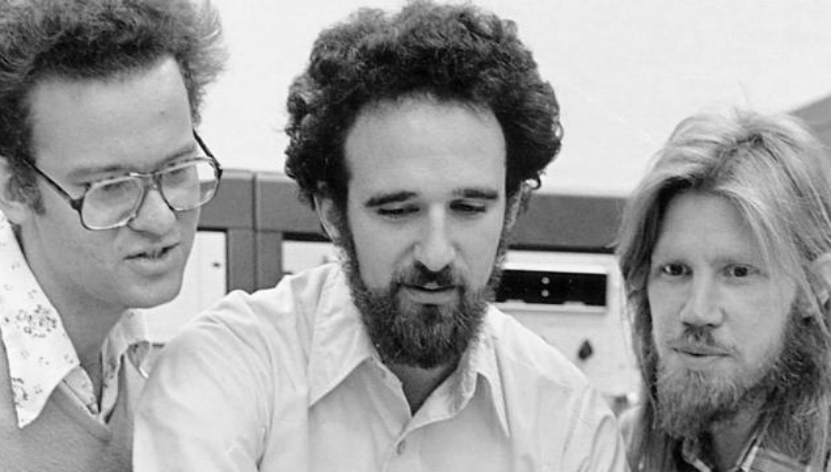
\includegraphics[width=91.77mm,height=130.38mm]{../../images/llm/page_002_img_01.png}%
\end{textblock*}

\end{document}
